\chapter{Descripción} \label{cap:Descripcion}
%\section{Descripción de la herramienta SLAM-Test-Bed} \label{s:descripcionHerramienta}
En este capítulo describiremos en detalle el funcionamiento de la herramienta SLAM-Test-Bed

La herramienta SLAM-Test-Bed consta de un entorno gráfico para realizar comparaciones sobre datasets obtenidos tras aplicar algoritmos SLAM. 
Nos permitirá medir la exactitud de los resultados de la aplicación de un algoritmo con los resultados de otro algoritmo o comparar varios resultados de un mismo algoritmo en el que se han aplicado distintos parámetros de ejecución.
La herramienta cuenta de un interfaz gráfico en 3D desarrollado en C++ con el entorno QT y la librería Eigen.


La aplicación sofware muestra al usuario un interfaz gráfico que permite:
Leer un archivo de datos con puntos 3D y mostrarlo en pantalla como una nube de puntos 3D. Este archivo podriamos denominarlo groundTruth.
\begin{figure}[H]
\begin{center}
\subfigure[]{\label{fig:Open File}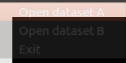
\includegraphics[height=2.0cm,width=6.0cm]{img/cap5/openFile.png}}
\hspace{0.5cm}
%\subfigure[]{\label{fig:LG_hombot}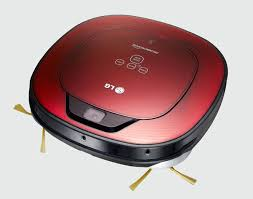
\includegraphics[height=6.0cm]{img/cap2/LG_hombot.jpg}}
\end{center}
%\caption{Robot Dyson 360 Eye (a) Robot Roomba 966 (b) Robot Hombot de LG (c).}
\caption{Selección de archivos de entrada }
\end{figure}

Con el ratón podremos girar en 3 dimensiones  la nube de puntos, acercarnos a el (Zoom in) o alejarnos (Zoom Out),
tambien permite leer un segundo conjunto de puntos 3D y estimar las transformaciones ( rotaciones , traslaciones, escala etc)  necesarias para pasar desde el conjunto de datos ground truth hasta este segundo conjunto de datos. El conjunto de datos resultante tras aplicar las estimaciones será visulalizado en pantalla como otra nube de puntos 3D

Esta herramienta poseé varios modulos accesibles desde el interfaz gráfico. Entre estos módulos podríamos destacar el \textbf{Módulo Transformador}.
Este módulo permite realizar transformaciones sobre el conjunto de puntos 3D groundTruth, de tal forma que se obtendrá como resultado una segunda nube de puntos transformados.
Los parámetros del módulo transformador serán accesible por pantalla
Entre las transformaciones permiten hacer cambios en :
\begin{itemize}
\item ESCALA
\item TRASLACIONES en ejes X,Y,Z
\item ROTACIONES en ejes X,Y,Z
\item Offset de tiempo
\item Interpolación
\item Ruido gaussiano
\item Ruido Cósmico
\end{itemize}

\begin{figure}[H]
\begin{center}
\subfigure[]{\label{fig:transformaciones}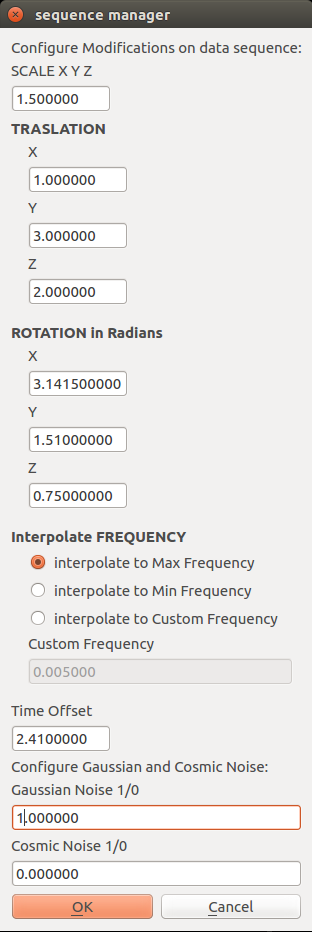
\includegraphics[height=12.0cm,width=4.0cm]{img/cap5/imgTransformaciones.png}}
\hspace{0.5cm}
%\subfigure[]{\label{fig:LG_hombot}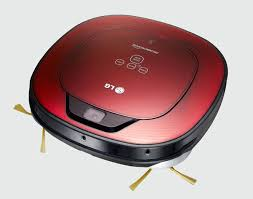
\includegraphics[height=6.0cm]{img/cap2/LG_hombot.jpg}}
\end{center}
%\caption{Robot Dyson 360 Eye (a) Robot Roomba 966 (b) Robot Hombot de LG (c).}
\caption{Detalle de la ventana de configuración de los parámetros de transformación }
\end{figure}


El formato del conjunto de datos ground-truth será timestamp, posición x, posición y, posición z, q0, q1 ,q2 ,q3 . Donde q0,q1,q2,q3 definen un quaternio.
A continuación un ejemplo de los datos de entrada:
\begin{figure}[H]
\begin{center}
\subfigure[]{\label{fig:data example}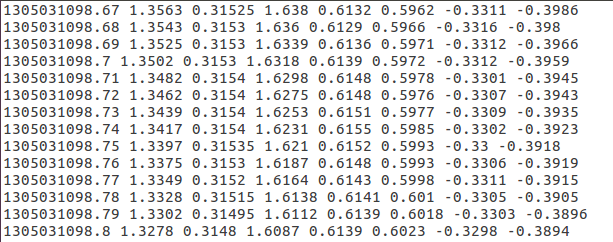
\includegraphics[height=3.0cm,width=8.0cm]{img/cap5/dataExample.png}}
\hspace{0.5cm}
%\subfigure[]{\label{fig:LG_hombot}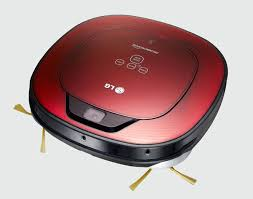
\includegraphics[height=6.0cm]{img/cap2/LG_hombot.jpg}}
\end{center}
%\caption{Robot Dyson 360 Eye (a) Robot Roomba 966 (b) Robot Hombot de LG (c).}
\caption{Ejemplo de los valores de los campo de cada registro del fichero de entrada. }
\end{figure}


Posteriormente tras aplicar las transformaciones definidas en el interfaz gráfico sobre el ground truth, la herramienta devolverá los resultados de estimar dichas transformaciones.


A continuación describiremos en detalle las transformaciones permitidas por la herramienta

\textbf{Escala}. Permite modificar los datos de entrada a nivel de escala. La escala siempre será mayor que cero y se admitirán números con reales

\textbf{Traslaciones}. Se podrán definir traslaciones sobre cada uno de los 3 ejes de coordenadas. 
La traslación admite números reales positivos y negativos.

\textbf{Rotaciones}. Se podrán definir rotaciones sobre cada unos de los 3 ejes de coordenadas. El valor de cada rotación se insertará en Radianes. Los valores admitidos serán números reales tanto positivos como negativos

\textbf{Offset de tiempo}. Con el offset de tiempo podremos introducir un gap en los valores de timestamp del fichero de entrada que más tarde podremos estimar. La exactitud del offset será de centésimas, es decir con 2 decimales

\textbf{Interpolación}: Se podrán realizar 3 tipos de interpolación de los datos.
	Interpolación a la frecuencia máxima
	Interpolación a la frecuencia mínima
	Interpolación a frecuencia personalizada

\textbf{Ruido Gaussiano}: Una de las transformaciones que podremos aplicar sobre el conjunto de datos del groundtrouth es aplicar un ruido gaussiano a los datos transformados

\textbf{Ruido Cósmico}: Otra transformación a aplicar sobre los datos transformados es la incorporación del ruido cósmico

\textbf{Menu de estimaciones}:


Una vez hemos aplicado las transformaciones sobre el groundtrouh, se generará como resultado un nuevo dataset, el transformado.
El menú gráfico nos permitirá estimar que transformaciones se han realizado, y se podrán estimar en 2 sentidos de aplicación, para ello deberemos utilizar el textbf{Módulo Estimador} accesible desde la barra de menú de SLAMTestBed

\begin{figure}[H]
\begin{center}
\subfigure[]{\label{fig:menu A to B y B to A}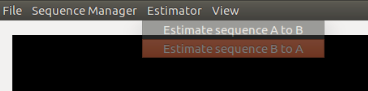
\includegraphics[height=3.0cm,width=8.0cm]{img/cap5/menuAtoB_BtoA.png}}
\hspace{0.5cm}
\end{center}
\caption{Transformaciones permitidas sobre el dataset de entrada }
\end{figure}
	Desde el groundtrouth estimar que transformaciones se han aplicado para llegar a la secuencia de datos transformados. ( A To B)

	Desde la secuencia transformada estimar las transformaciónes para obtener el groundtrouth . ( B to A)
Estas 2 estimaciones se han realizado aplicando cálculos matemáticos tipo SVD y PCA sobre las matrices de datos.
Tambien existe la posiblidad de realizar estas estimaciones transformaciónes utilizando el algortimo RANSAC
Al terminar de calcular las estimaciones aparecerá una ventana con los resultados de las estimaciones calculadas
\begin{figure}[H]
\begin{center}
\subfigure[]{\label{fig:Transformaciones versus Estimaciones}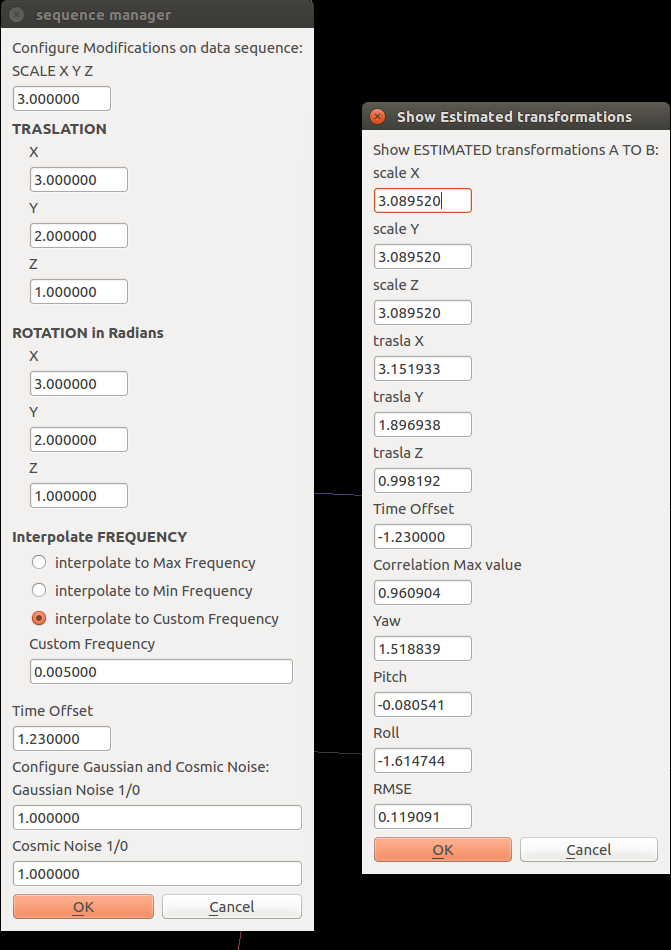
\includegraphics[height=12.0cm,width=8.0cm]{img/cap5/showTransformationsEstimated.png}}
\hspace{0.5cm}
\end{center}
\caption{Transformaciones realizadas frente Transformaciones estimadas }
\end{figure}


\begin{figure}[H]
\begin{center}
\subfigure[]{\label{fig:menu A to B RANSAC}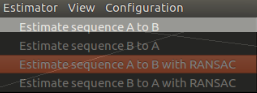
\includegraphics[height=3.0cm,width=8.0cm]{img/cap5/menuEstimatorRANSAC.png}}
\hspace{0.5cm}
%\subfigure[]{\label{fig:LG_hombot}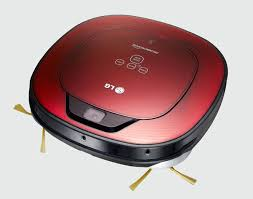
\includegraphics[height=6.0cm]{img/cap2/LG_hombot.jpg}}
\end{center}
%\caption{Robot Dyson 360 Eye (a) Robot Roomba 966 (b) Robot Hombot de LG (c).}
\caption{Transformaciones permitidas con RANSAC sobre el dataset de entrada }
\end{figure}


\textbf{Otras particularidades del menú gráfico}:
La barra de menu de SLAMTestbed, tambien tiene el elemento \textbf{View}. Este elemento de menu ofrece varias opciones gráficas a aplicar sobre los puntos 3D de los conjuntos, y estas son:
\begin{figure}[H]
\begin{center}
\subfigure[]{\label{fig:opciones de View}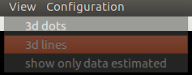
\includegraphics[height=3.0cm,width=8.0cm]{img/cap5/dotsAndLines.png}}
\hspace{0.5cm}
%\subfigure[]{\label{fig:LG_hombot}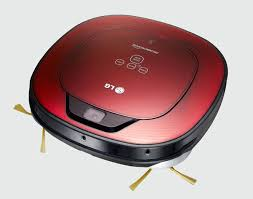
\includegraphics[height=6.0cm]{img/cap2/LG_hombot.jpg}}
\end{center}
%\caption{Robot Dyson 360 Eye (a) Robot Roomba 966 (b) Robot Hombot de LG (c).}
\caption{Transformaciones permitidas con RANSAC sobre el dataset de entrada }
\end{figure}
\textbf{Unir con lineas todos los puntos de cada dataset}. Esta opción es especialmente util cuando estemos utilizando ruido cósmico, ya que al unir los puntos con líneas podremos ver con claridad los puntos con elevado nivel de ruido, que deberían ser tratados como outliers.

\begin{figure}[H]
\begin{center}
\subfigure[]{\label{fig:opciones de View}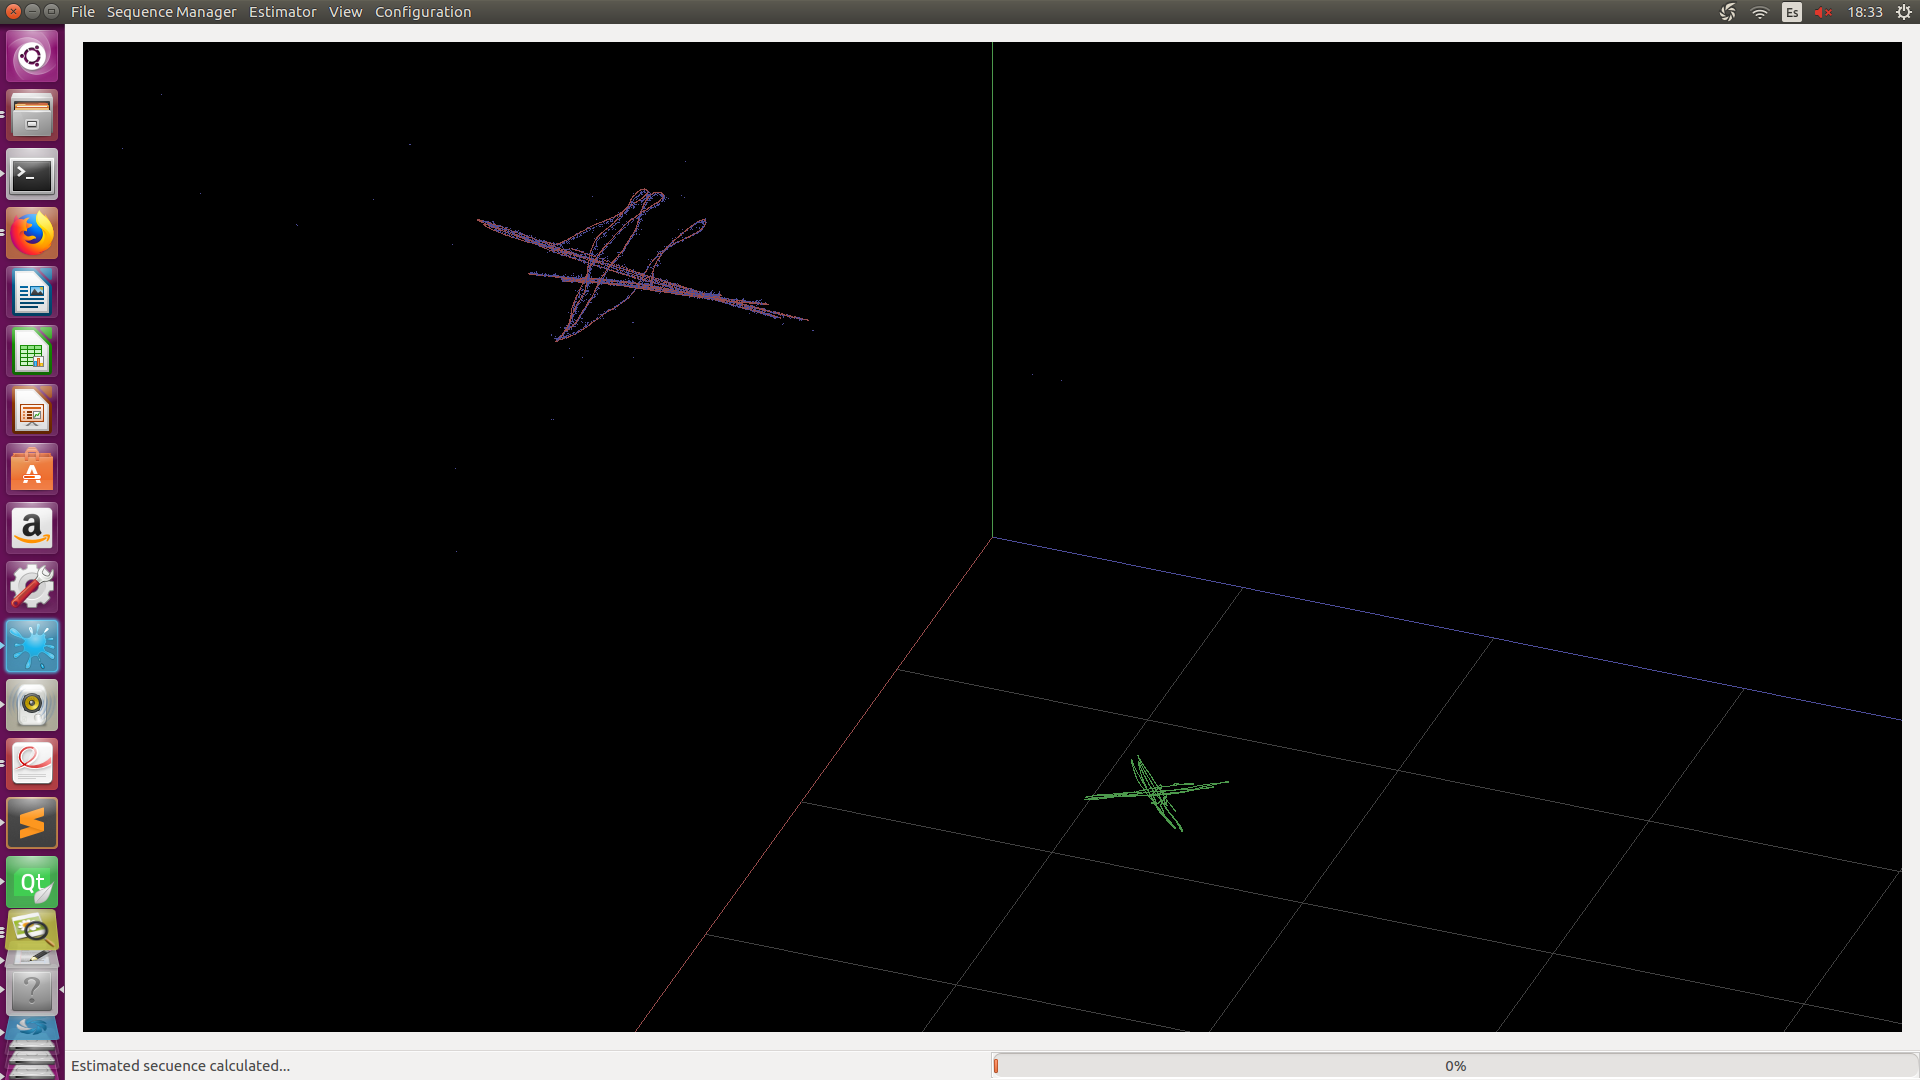
\includegraphics[height=5.0cm,width=10.0cm]{img/cap5/3dDots.png}}
\hspace{0.5cm}

\end{center}

\caption{Ejemplo de datasets visualizados como puntos 3D. Los puntos con ruido cósmico apenas se aprecian. }
\end{figure}


\begin{figure}[H]
\begin{center}
\subfigure[]{\label{fig:opciones de View}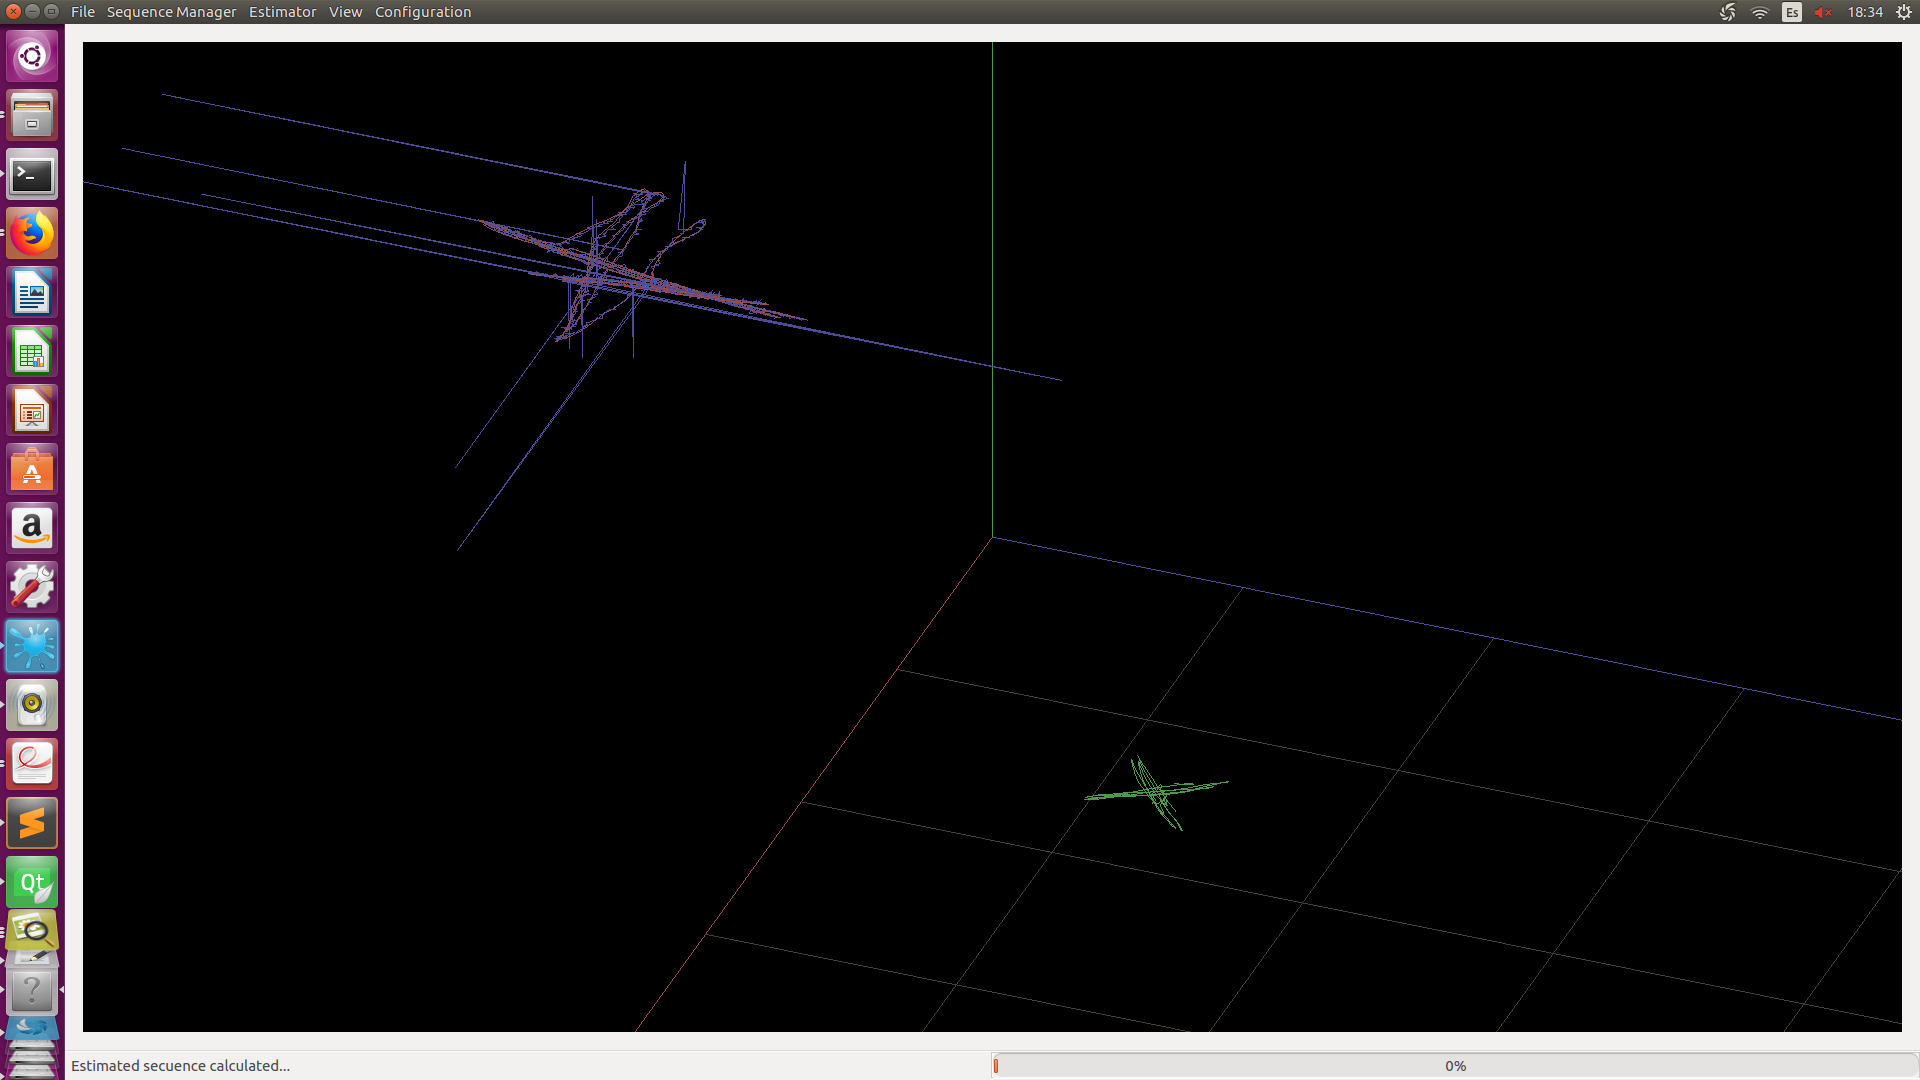
\includegraphics[height=5.0cm,width=10.0cm]{img/cap5/3dLines.png}}
\hspace{0.5cm}

\end{center}

\caption{Ejemplo de datasets visualizados como líneas 3D donde se aprecian mejor los puntos con ruido cósmico}
\end{figure}

Las opciones del menú View tambien permiten sólo visualizar los puntos 3D resultado de las transformaciones estimadas.

    
La explicación del algoritmo:
En este apartado explicaremos los pasos seguidos para hacer los calculos que nos permitiran estimar las transformaciones requeridas para pasar de un dataset A a otro dataSet B
Las principales funciones o módulos de los que constará la herramienta será:
\begin{description}
\item [Cálculo de PCA]: Nos permitirá reducir el dataset a  sus componentes principales
\item [Estimación de Escala]: Estimará la diferencia de escala entre los dos datasets
\item [Estimación de Offset]: Con este módulo podremos hallar la diferencia entre marcas de tiempos de los 2 datasets
\item [Interpolación para igualar frecuencias de muestreo]: Con la interpolación podremos igualar en frecuencias los dos datasets
\item [Operaciones de Registro para estimar la Rotación y Traslación]: Permitirá estimar las traslación y rotación necesarias para pasar de un datasetA a un datasetB
\end{description}


\begin{figure}[H]
\begin{center}
\subfigure[]{\label{fig:opciones de View}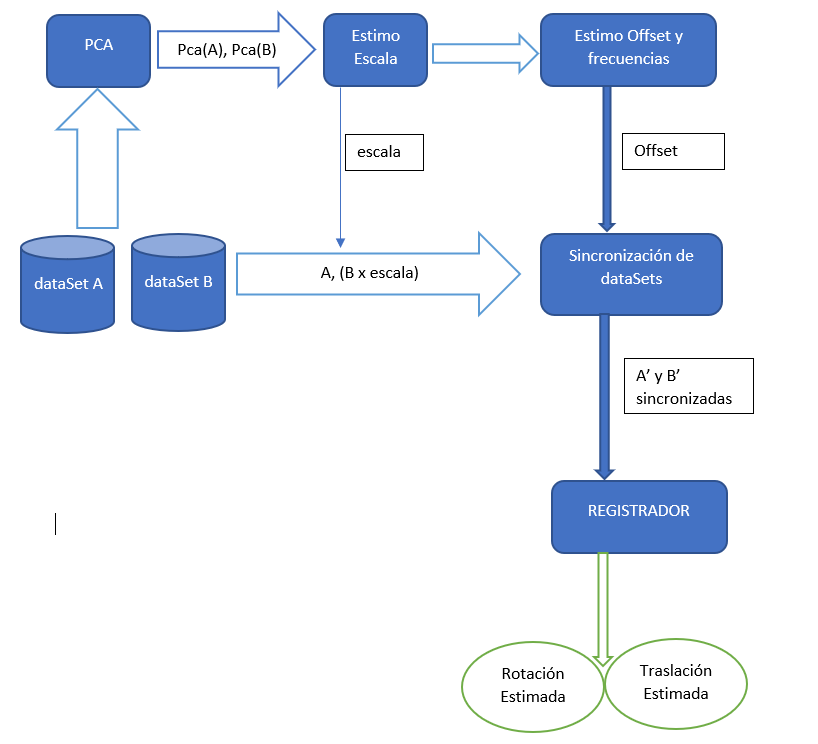
\includegraphics[height=8.0cm,width=12.0cm]{img/cap5/esquemaTFM.PNG}}
\hspace{0.5cm}

\end{center}

\caption{Esquema del algoritmo seguido para estimar las transformaciones.}
\end{figure}

ESCRITURA DE LOS ALGORITMOS


Cuando tengamos un DatasetA y un DataSetB, el algoritmo que seguiremos para estimar las transformaciones desde el DatasetA al DataSetB serán las siguientes.

Calcular PCA para cada dataset, con estos nuevos datasets, calularemos la escala. Posteriormente estimaremos el offset de tiempo entre los dos datasets y unificaremos las 
frecuencias

Con los datos dataSetApca y dataSetBpca estimaremos el offset de tiempo que hay entre las 2 secuencias de datos o datasets
Posteriormente corregiremos el offset en el dataset B, para ello sumaremos el valor del offset a los valores de tiempo del datasetB
Una vez tengamos calculado el offset, unificaremos las frecuencias de los 2 datasets mediante interpolación.
Cuando tengamos unificada la frecuencia para los dos datasets, obtendremos de nuevo PCA de cada dataset y por último obtendremos la escala.

Posteriormente estimaremos  la transformaciones de rotación y traslación para pasar del datasetA al datasetB
Aplicaremos dichas transformaciones sobre el datasetA , lo que nos dará como resultado un nuevo dataset, el dataset Estimado que pintaremos en pantalla de color rojo

Cálculo del offset:
Este módulo se encarga de estimar el offset o diferencia de tiempo entre los dos datasets. Es el algoritmo más pesado ya que incluye múltiples cálculos para interpolar y calcular 
la correlación cruzada entre los dos datasets.

Este algoritmo será iterativo en el que utilizaremos un dataset como base de tiempo fijo y otro dataset B que se deslizará en el tiempo desde -T hasta +T . El datasetB se irá 
deslizando en pequeños espacios de tiempo o steps en cada iteración. Para cada step calcularemos la correlación cruzada entre el dataset deslizante y el dataset original(que se 
mantiene fijo en el tiempo). Para un step determinado la correlación debe ser máxima entre los 2 datasets y cuando hallemos la correlación máxima, el step de esa iteración nos 
indicará el offset. Como hemos comentado, moveremos el datasetB a -T y por cada iteración iremos deslizando en el tiempo el datasetB un incremento de tiempo step , hasta el final 
del bucle que terminaremos de deslizar datasetB hasta +T. En cada iteracción calcularemos la interpolación en los puntos que coincidan que esten dentro de los límites de los dos 
datasets.Una vez interpoladas los puntos comunes de las 2 series tendremos 2 series nuevas, Para las cuales calcularemos la crosscorrelación cruzada aplicando el algoritmo típico 
para 2 series temporales.Pero antes, y como cada serie temporal tiene 3 coordenadas (x,y,z para cada punto 3d), debemos transformar estas 3 coordenadas en un sólo valor para cada 
punto 3D de cad serie, para ello para cada punto 3D calcularemos su distancia al origen , y por tanto la correlación cruzada se calculará sobre las 2 datasets convertidos a 
distancias al origen de coordenadas.

\begin{figure}[H]
\begin{center}
\subfigure[]{\label{fig:opciones de View}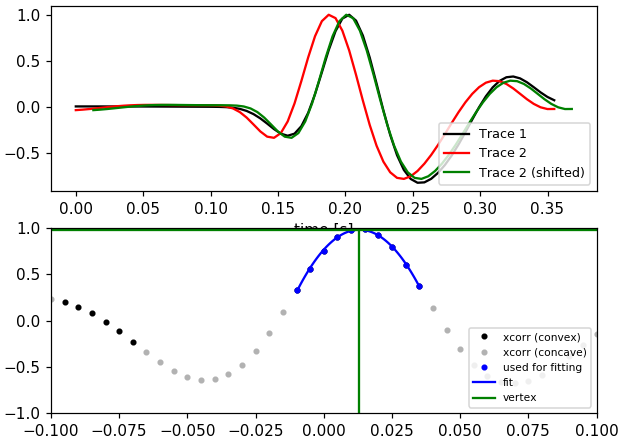
\includegraphics[height=8.0cm,width=12.0cm]{img/cap5/correlacionCruzada.png}}
\hspace{0.5cm}

\end{center}

\caption{Gráfico que muestra el desfase del offset entre dos series temporales y el resultado de la correlación cruzada.}
\end{figure}

Acontinuación describiremos cada unos de los módulos que componen la herramienta SLAMTestBed.
\begin{enumerate}%for small alpha-characters within brackets.


\item \textbf{El módulo Ajuste de Tiempo:}

	Con este módulo podremos calcular el offset de tiempo entre los 2 datasets.
	El método principal utilizado para calcular el offset se realiza mediante el calculo de la Cross Correlación Cruzada
	Para ello previamente , calcularemos la distancia al origen para cada punto 3D de los 2 datasets
	Para un punto 3d (x,y,z), la distancia 3d se calculará 
	\begin{math}
	\sqrt{(x-0)^2 +(y-0)^2+(z-0)^2}
	\end{math}
	una vez calculadas las distancias , aplicaremos el siguiente algoritmo de calculo de correlación cruzada
	                                
	
									   dataA = CalcularDistancia( dataSetA)

									   dataB = CalcularDistancia( dataSetB)

									   mA = CalcularMedia(dataA)

									   mB = CalularMedia(dataB)

									   Para cada fila

									   		sx = dataA(i) - mA

									   		sy = dataB(i) - mB

								       denom = \begin{math}\sqrt{sx*sy}\end{math};

									   step = 0.01		

								       Desde i=-T hasta i = T

								            Si ( dataB.t < dataB.t )

								            	j=j+1

								            	continuar

								            sino si (dataB.t > dataA.t)

								            	i=i+1

								            	continuar

								            	sino si (dataB.t == dataA.t)

								            		sxy=(dataA -mA) * (dataB-mB)

								            		i++

								            		j++

								       

								       r = (sxy) / denom;

								       r= fabs(r);


	   	
	

\item \textbf{El módulo Generator PCA:}

	Con el módulo PCA obtendremos las componentes principales de un dataset, generando un nuevo dataset.

	A partir de los nuevos datasets generados podremos calcular la escala y la diferencia de tiempos entre los 2 datasets.

	Se implementan 2 métodos de cálculo de PCA, el segundo utilizando el método SVD (utilizando la librería Eigen), que describiremos acontinuación.

		
		\textit{mX= media (dataset.x)}

		\textit{mY= media (dataset.y)}

		\textit{mZ= media (dataset.z)}

	    \textit{restar la media a cada componente x, y z}

	    \textit{dataset.x = dataset.x - mX } 

	    \textit{dataset.y = dataset.y - mY }

	    \textit{dataset.z = dataset.z - mZ }

	    \textit{cov = obtenerMatrizCovarianza(dataset)}

	    \textit{svd = CalularSVD(cov )}

	    \textit{pca =  Matriz V del resultado svd}

	    \textit{datasetResultado = dataset * Matriz (svd.V)}
	    

		


\item \textbf{El módulo Interpolador:}

	El módulo de interpolación se utiliza para sincronizar a igual frecuencia 2 datasets.
	Entre las distintas funciones , permite sincronización a la frecuencia mayor de los 2 datasets, sincronización a la frecuencia menor de los 2 datasets o incluso consigue sincronizar las 2 series a una frecuencia deseada. La interpolación se realiza sobre las secuencias temporales de los 2 datasets, pero tambien se calcula la interpolación para las coordenadas X,Y y Z de cada punto 3D y se realiza tambien interpolación para los quaternios. La función \textit{slerp} de la librería Eigen nos permite calcular la interpolación entre quaternios. La función slerp recibe como parámetro una marca de tiempo y un quaternio.

\item \textbf{El módulo Escala:}

Nos permitirá calcular la diferencia de escala entre los dos datasets.
El algoritmo utilizado será utilizando los valores singulares de cada datasets.
        
	
		\textit{S1 = svd(dataSet1).valoresSingulares}

	    \textit{S2 = svd(dataSet2).valoresSingulares}

	    \textit{scalaX = S2(0)  / S1(0) }

	    \textit{scalaY = S2(1)  / S1(1) }

		\textit{scalaZ = S2(2)  / S1(2) }
		



\item \textbf{El módulo Registrador:}

El módulo Registrador nos permitirá estimar las transformaciones (Rotación y Traslación) para pasar del dataSetA al dataSetB y viceversa
Entre las funciones que nos permitirá este módulo destancan:
    \begin{description}
	\item [Hallar la matrices de rotación y traslación] .

		El algoritmo para esta funcionalidad sería el siguiente:

        \textit{
		- Hallar los centroides de las coordenadas X,Y,Z de cada dataset
		  centA = centroides (A)
          centB = centroides (B)
        }

        \textit{
        - Restar los centroides a sus respectivas matrices
          A= A-centA
          B= B-centB
        }

        \textit{
        - Calcular el producto de las matrices}

        \textit{
          H = A.traspuesta * B
        }

        \textit{
        - Obtener la descomposición en valores singulares de la matriz H
        }

        \textit{
          S,U,V = svd(H) }
        
        \textit{
        - Obtener la matriz de Rotación}

        \textit{
          R = V*U.traspuesta}

        \textit{
        - Obtener la matriz de Traslación}

        \textit{ 
          t= -R * centA + centB;  
        }

	\item[Transformar un dataset en otro aplicando las matrices de Rotación y Traslación previamenete estimadas]

		Este método tomará un dataset , lo multiplicará por la matriz de rotación y le sumará la matriz de traslación.

	\item[Transformar los cuaternios aplicando la matriz Rotación.]

		Con este método conseguimos transformar los cuarternios del dataSetA al dataSetB.
		Para ello convertiremos la matriz de rotación en un cuaternio que llamaremos "q".
		Por último multiplicaremos cara quaternio p de la siguiente forma.
		  q * p * q.inverso 

	\item[Estimar las matrices de rotación y traslación mediante la técnica de RANSAC.]

		Estimaremos las matrices de Rotación y Traslación utilizando los datos de los 2 datasets.

		El algoritmo seguido ha sido el siguiente:
         
	        \textit{Mientras no alcancemos el número máximo de iteraciones hacer}

		    	\textit{		Seleccionar n inliers}

				\textit{		Estimar una primera matriz de Rotación , traslación}

		        \textit{		aplicar transformación sobre un subconjunto de puntos No Inliers}

		        \textit{		Si el error < threshhold}

					\textit{			añadir cadidato a inliers}

				\textit{		medir el error tras aplicar transformaciones sobre inliers y no inliers}

				\textit{		seleccionar menor error}

			 	\textit{		incrementar iteracción}


	        
	        \textit{Devolveremos las matrices de Rotación Traslación que menor error hayan dado}     
	        

    \end{description}


\item \textbf{El módulo Transformador:}
	Con este nos permitirá crear a partir de un dataset original , un segundo dataset modificado, que será el resultado de realizar varias transformaciones sobre el primer dataset
	Con la función createContaninatedSequence podremos realizar todas o algunas de las siguientes modificaciones sobre el dataset original
		- Cambio de escala

		- aplicar una Rotación

		- aplicar una Trasalación

		- aplicar un desplazamineto en el tiempo, (offset)

        - Realizar cambios en la frecuencia

        - Introducir ruido Gaussiano en los datos

        - Introducir ruido Cósmico


\item \textbf{El módulo Estadísticas:}

	Este módulo permite calcular el Error Cuadrático Medio (Root Mean Square Error) entre 2 datasets.

\end{enumerate}



